\begin{figure}[htbp]
    \centering
    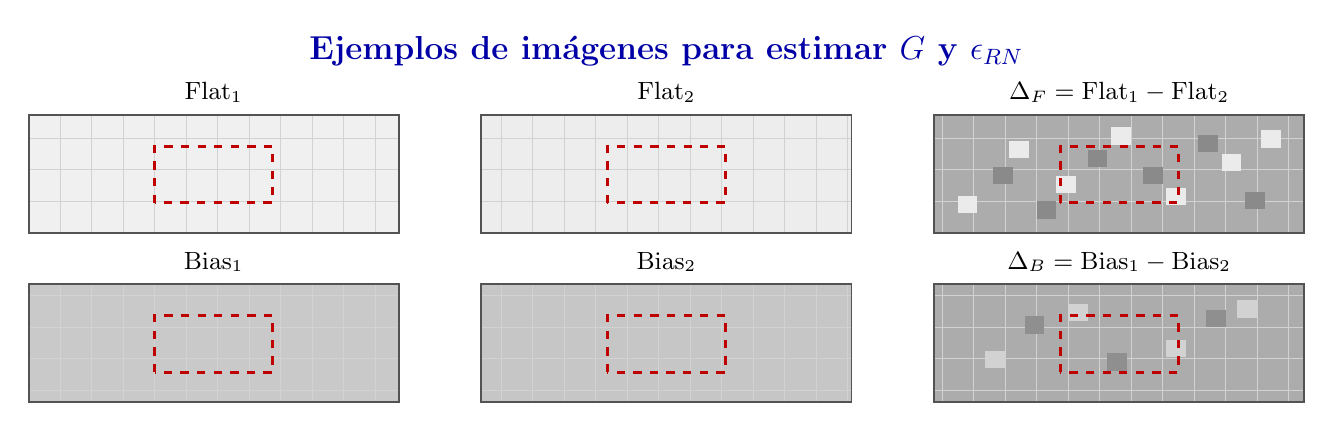
\begin{tikzpicture}[
        font=\small,
        region/.style={draw=red!75!black, dashed, line width=1pt},
        borde/.style={draw=gray!65!black, line width=0.7pt}
    ]
        \node[font=\bfseries\large, text=blue!65!black] at (8.5,4.3)
            {Ejemplos de imágenes para estimar $G$ y $\epsilon_{\text{RN}}$};

        \node[font=\small\bfseries] at (2.75,3.78) {$\mathrm{Flat}_1$};
        \node[font=\small\bfseries] at (8.5,3.78) {$\mathrm{Flat}_2$};
        \node[font=\small\bfseries] at (14.25,3.78)
            {$\Delta_F=\mathrm{Flat}_1-\mathrm{Flat}_2$};
        \node[font=\small\bfseries] at (2.75,1.63) {$\mathrm{Bias}_1$};
        \node[font=\small\bfseries] at (8.5,1.63) {$\mathrm{Bias}_2$};
        \node[font=\small\bfseries] at (14.25,1.63)
            {$\Delta_B=\mathrm{Bias}_1-\mathrm{Bias}_2$};

        % Matrices esquemáticas: tonos uniformes para frames originales
        \foreach \xa/\xb/\ya/\yb/\tono in {
            0.4/5.1/2.0/3.5/gray!12,
            6.15/10.85/2.0/3.5/gray!14,
            11.9/16.6/2.0/3.5/gray!65,
            0.4/5.1/-0.15/1.35/gray!42,
            6.15/10.85/-0.15/1.35/gray!45,
            11.9/16.6/-0.15/1.35/gray!65
        } {
            \fill[\tono] (\xa,\ya) rectangle (\xb,\yb);
            \draw[step=0.4cm, draw=gray!35, line width=0.2pt]
                (\xa,\ya) grid (\xb,\yb);
            \draw[borde] (\xa,\ya) rectangle (\xb,\yb);
        }

        % Fluctuaciones de píxel a píxel en las imágenes diferencia
        \foreach \x/\y in {
            12.2/2.25, 12.85/2.95, 13.45/2.5, 14.15/3.12,
            14.85/2.35, 15.55/2.78, 16.05/3.08
        } {
            \fill[gray!16] (\x,\y) rectangle ++(0.25,0.22);
        }
        \foreach \x/\y in {
            12.65/2.62, 13.2/2.18, 13.85/2.83, 14.55/2.62,
            15.25/3.02, 15.85/2.3
        } {
            \fill[gray!92] (\x,\y) rectangle ++(0.25,0.22);
        }
        \foreach \x/\y in {12.55/0.28, 13.6/0.88, 14.85/0.42, 15.75/0.92} {
            \fill[gray!35] (\x,\y) rectangle ++(0.25,0.22);
        }
        \foreach \x/\y in {13.05/0.72, 14.1/0.25, 15.35/0.8} {
            \fill[gray!88] (\x,\y) rectangle ++(0.25,0.22);
        }

        % Misma región central de medida en cada frame
        \foreach \x in {2.0,7.75,13.5} {
            \draw[region] (\x,2.38) rectangle ++(1.5,0.72);
            \draw[region] (\x,0.23) rectangle ++(1.5,0.72);
        }
    \end{tikzpicture}
    \caption{Representación ilustrativa, no basada en datos reales, de dos
    flats y dos bias junto con sus imágenes diferencia. El contorno discontinuo
    señala la misma región central usada para medir medias y dispersiones;
    las diferencias muestran las fluctuaciones píxel a píxel.}
    \label{fig:imagenes-flat-bias}
\end{figure}